\section{Three-tier architecture}

\begin{figure}[H]
    \centering
    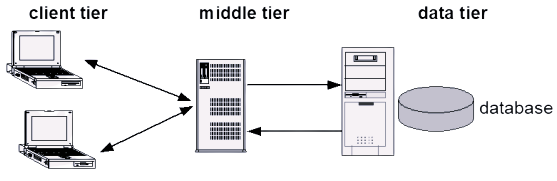
\includegraphics[width=0.5\linewidth]{images/tt.png}
    \caption{Three-tier architecture}
\end{figure}
The hardware used by the three-tier architecture is: 
\begin{itemize}
    \item Server for data management. 
    \item Client for presentation layout. 
    \item Middle tier to achieve a better separation between the client and the server. 
\end{itemize}
This architecture has several variants, depending on the software features of the middle tier. 

\subsection*{Web pure HTML three-tier architecture}
\begin{figure}[H]
    \centering
    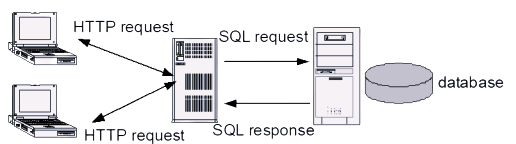
\includegraphics[width=0.5\linewidth]{images/ttph.png}
    \caption{Web pure HTML three-tier architecture}
\end{figure}
In the pure HTML architecture the client is a standard web browser, and it has to cope with the presentation layout only (thin client). The middle tier: 
\begin{itemize}
    \item Includes a Web server that exploits HTTP.
    \item Hosts the business logic for dynamically generating content from the raw data of the data tier. 
    \item Deals with the presentation layout. 
\end{itemize}

\subsection*{Rich internet applications}
\begin{figure}[H]
    \centering
    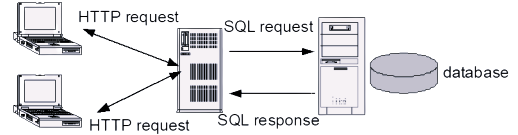
\includegraphics[width=0.5\linewidth]{images/ttria.png}
    \caption{Rich internet applications three-tier architecture}
\end{figure}
The rich internet application architecture is the fusion of web and desktop applications (with JavaScript). 
In this case the client is called fat because it has standard communication protocol (HTTP, Web Socket), language (ECMAScript) and API (DOM, HTML5). 
The features of this architecture are: 
\begin{itemize}
    \item New interface event types, also specific to touch and mobile apps.
    \item Asynchronous interaction (AJAX).
    \item Client-side persistent data.
    \item Offline applications.
    \item Native multimedia and 3D support.
\end{itemize}